\section{Introduction}
\label{Introduction}
%The isocenter of the magnetic gradient fields inside a Magnetic Resonance (MR) Imaging scanner is used in many distortion correction methods for MR images~\cite{Dor05,LSS06a,LSS06b,LSS08a,tlee_iaeng,simple_approach,Wang04a,Wang04b}.  Currently there is no known method for estimating the gradient isocenter. All existing estimation methods are using the DICOM patient center which is very close but not exactly the same as isocenter. The different between isocenter and DICOM patient center could contribute part of the error of overall correctness of estimation.

Magnetic resonance imaging (MRI) provides an excellent modality for distinguishing different tissues in the human body, which makes this modality essential for medical applications. MRI can also be used for treatment planning of medical procedures that require a great degree of geometrical accuracy such as  functional radiosurgery~\cite{Kond99}. Unfortunately, the accuracy of MRI for medical targeting applications is compromised by the presence of geometric distortions such as non-linearities of the magnetic gradient fields or inhomogeneities of the scanner main field ~\cite{Dor05,LSS06a,LSS06b,LSS08a,tlee_iaeng,simple_approach,Wang04a,Wang04b}. Gradient nonlinearities can cause over 2mm of distortion to the location of features in the image~\cite{tlee_iaeng,simple_approach}.

Modern MRI scanners have built-in distortion correction algorithms, that rely on knowledge of the magnetic field configuration and its distortion. Built-in algorithms, which are usually proprietary, are designed based on assumed knowledge of the geometry and location of the gradient coils. A more practical approach is to use a phantom of known geometry and to derive the distortion by analyzing the MRI images generated with such a phantom ~\cite{Dor05,LSS06a,LSS06b,LSS08a,tlee_iaeng,simple_approach,Wang04a,Wang04b}. This method has the advantage that a scanner-specific correction can be applied, which can also take into account potential changes in the gradient fields over time.

Accurate knowledge of the gradient isocenter is essential to very accurate distortion correction methods, To our knowledge, existing distortion correction algorithms, both built-in and phantom based, make the assumption that the gradient isocenter coincides with the origin of the DICOM coordinates. This assumption may not be accurate and should not be used if a high degree of accuracy is necessary.

The goal of this work was to develop and implement a numerical software-based method to estimate the gradient isocenter of the magnetic field inside an MRI scanner using the MRI scan of a custom-built phantom.  In our previous work~\cite{LSS06a,LSS06b,LSS08a,tlee_iaeng}, we used an oil filled plexiglass cube with
159.50mm $\times$ 159.70mm $\times$ 158.11mm dimension that was designed to fit MR scanners that were available at that time.  Current MRI scanners have a significantly wider aperture, which necessitates a larger phantom to characterize the field distortion.  Furthermore, since the lower part of the scanner aperture is occupied by the scanner table, the scanning area occupied by the phantom or the patient is not centered on the gradient isocenter, making correction methods that assume that the phantom is centered with respect to the gradient isocenter~\cite{LSS06a,LSS06b,LSS08a,tlee_iaeng,simple_approach} obsolete and potentially inaccurate.

\section{Distortion Phantom}
A new phantom design was developed with the intention to probe the distortion in the 50 cm field-of-view (FOV) of a modern 3T MRI scanner (Magnetom Trio, Siemens).  Due to the geometry of the gradient field nonlinearity, the distortion is largest in the outer fringes of the FOV~\cite{LSS06a,LSS06b,LSS08a,tlee_iaeng}. Capturing distortion data in the periphery of the FOV is important for better accuracy of the distortion correction. Building a very large cubical oil-filled phantom is a challenge due to weight limitations and limited capability to accurately machine a very large flat surface. Thus it was felt to be impractical to simply scale up the original phantom.  Another limitation is that the phantom needs to fit inside the scanner head coil which needs to be used to achieve a sufficiently high signal-to-noise ratio.  To meet all requirements, we designed a phantom that is comprised of 64 NMR glass tubes of 3 mm inner diameter, filled with copper sulfate and arranged in 8 surfaces forming an octagon.  A water-filled cylinder in the middle of the octagon ensures a good signal generated by the tubes.  The distance between tubes on the opposite side of the surface is 205mm, which is about 28\% wider than the original phantom. In addition we also added four more surfaces to provide data and better fit the headcoil.  There are 8 removable tubes on each surface with 10 mm gap between adjacent tubes.  Each tube is about 207 mm long, which is also an increase of about 28\% in length from the original phantom.  Tubes are placed along the main axis of the magnetic $B_0$  field to reduce the effects of chemical shift and magnetic susceptibility and
resulting in high-quality axial images.

\section{Computational Algorithm}

The algorithm we described here is using simulated data set that is based the
geometric property of the phantom and the properties of the MR images.
The MR images we are using have 1mm per pixel resolution for every image and
1mm thickness between two adjacent planes. In the simulation, we will be using millimeters as unit for
each data point. Since the images we are using to collect data points are all axial scans,
we will only add noise to x and y coordinate of each data point.

\section{Tube Modeling}

The tubes are 203 mm long. So our simulation data is ranging from -100 to 100 on z axis for each tube.
The arrangement of the tubes could be seen in Figure~\ref{fig:1}.
Our algorithm is based on two standard assumptions~\cite{LSS06a,LSS06b,LSS08a,tlee_iaeng,simple_approach}.: (1) the distortion in MR images are only caused by the magnetic field inside MRI scanner and (2) the magnetic field can be perfectly described using the sum of spherical harmonic.

\begin{figure}[htb]

  \begin{minipage}[b]{2.2in}
    \centering
    \centerline{\mbox{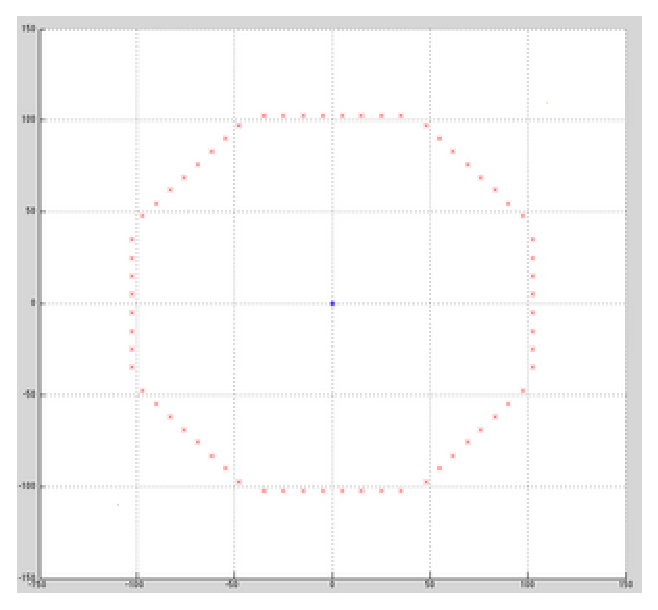
\includegraphics[width=2.2in]{isocenter/images/simulation/axial_no_distortion.eps}}}
    \centerline{\emph{(a) Axial view.}}
  \end{minipage}
  \hfill
  \begin{minipage}[b]{2.2in}
    \centering
    \centerline{\mbox{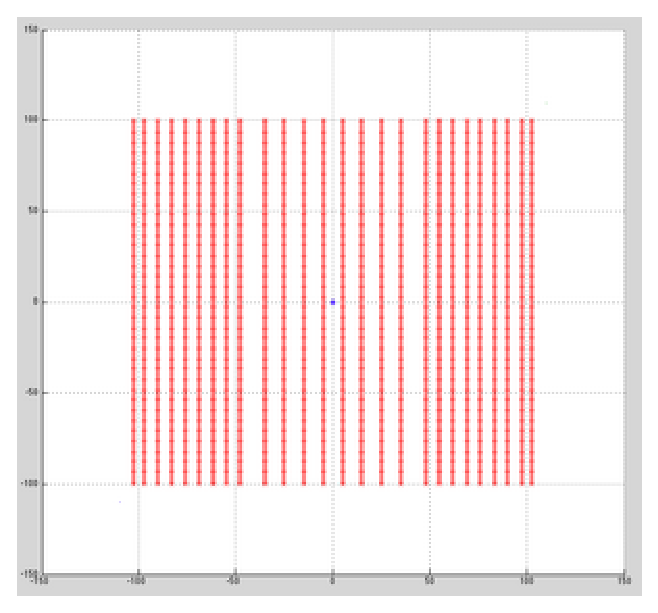
\includegraphics[width=2.2in]{isocenter/images/simulation/coronal_no_distortion.eps}}}
    \centerline{\emph{(b) Coronal view.}}
  \end{minipage}
%\hfill
%
  \caption{Phantom modeling without distortion} 
  \label{fig:1}
%
\end{figure}

The spacial coordinate of the phantom must be transformed into a coordinate relative to the gradient isocenter
of the magnetic field, see Equation~\ref{eq1}, then using the first 5 terms of the spherical harmonic we can estimate
a offset in $x$, $y$, $z$ direction, see Equation~\ref{eq2}. Finally this offset is added the original coordinate
to create a distorted model, see Equation~\ref{eq3}.  Also a very key requirement for this algorithm is that the z-axis the phantom which is parallel to the tubes must be aligned with the z-axis of the magnetic field.

\begin{eqnarray}
\begin{bmatrix}
x^\prime  \\
y^\prime  \\
z^\prime  \\
\end{bmatrix}
& = &
\begin{bmatrix}
x \\
y \\
z \\
\end{bmatrix}
-
\begin{bmatrix}
x_{iso} \\
y_{iso} \\
z_{iso}\\
\end{bmatrix}
\label{eq1}
\\
K & = &
\begin{bmatrix}
K_{x_0} \; K_{x_1} \; K_{x_2} \; K_{x_3} \; K_{x_4} \\
K_{y_0} \; K_{y_1} \; K_{y_2} \; K_{y_3} \; K_{y_4} \\
K_{z_0} \; K_{z_1} \; K_{z_2} \; K_{z_3} \; K_{z_4} \\
\end{bmatrix}
\\
\begin{bmatrix}
\alpha \\
\beta \\
\zeta \\
\end{bmatrix}
& = &
K
\begin{bmatrix}
{x^\prime}^2 + {y^\prime}^2 \\
{z^\prime}^2 \\
{z^\prime}^2 {({x^\prime}^2 + {y^\prime}^2)}^2 \\
{({x^\prime}^2 + {y^\prime}^2)}^2 \\
{z^\prime}^4 \\
\end{bmatrix}
\end{eqnarray}
\begin{eqnarray}
\begin{bmatrix}
  \Delta x \\
  \Delta y \\
  \Delta z \\
\end{bmatrix}
& = &
\begin{bmatrix}
x^\prime \alpha \\
y^\prime \beta \\
z^\prime \zeta \\
\end{bmatrix}
\label{eq2}
\\
\begin{bmatrix}
\bar{x} \\
\bar{y} \\
\bar{z} \\
\end{bmatrix}
& = &
\begin{bmatrix}
x + \Delta x \\
y + \Delta y \\
z + \Delta z \\
\end{bmatrix}
\label{eq3}
  % \bar{\alpha_i} & = & \alpha_i \left(1+  K_{\alpha_0} \left((x_i - ISO_x)^2 + (y_i - ISO_y)^2 \right)  \right. \nonumber\\
  % &&\qquad      \left.    + K_{\alpha_1}(z_i - ISO_z)^2 \right. \nonumber\\
  % &&\qquad      \left.    + K_{\alpha_2}(z_i - ISO_z)^2 \left((x_i - ISO_x)^2 + (y_i - ISO_y)^2 \right)  \right. \nonumber\\
  % &&\qquad      \left.    + K_{\alpha_3} \left((x_i - ISO_x)^2 + (y_i - ISO_y)^2 \right)^2 \right. \nonumber\\
  % &&\qquad      \left.    + K_{\alpha_4}(z_i - ISO_z)^4 \right)
% \label{eq6}
\end{eqnarray}

\section{ISO-Center Coordinate Estimation}

Using a exaggerated distortion parameter we can visualize the shape of the distortion model. Without distortion, the phantom appears as in Figure~\ref{fig:1}.  With large distortions, the phantom appears as in Figure~\ref{fig:2}, which is useful to understand the form of the distortions.  A more realistic distortion can be seen in Figure~\ref{fig:3}, which uses distortion parameters from~\cite{tlee_iaeng}.


\begin{figure}[htb]

  \begin{minipage}[b]{1.65in}
    \centering
    \centerline{\mbox{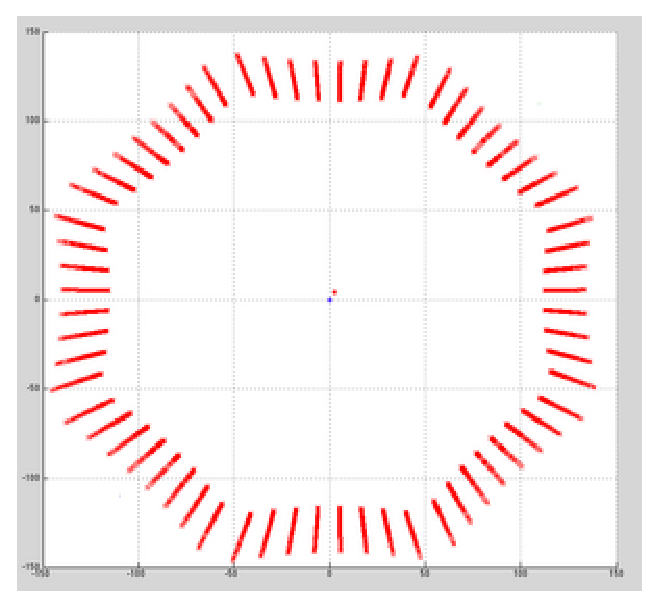
\includegraphics[width=1.65in]{isocenter/images/simulation/axial_distortion_0.eps}}}
    \centerline{\emph{(a) Axial view.}}\medskip
  \end{minipage}
  \hfill
  \begin{minipage}[b]{1.65in}
    \centering
    \centerline{\mbox{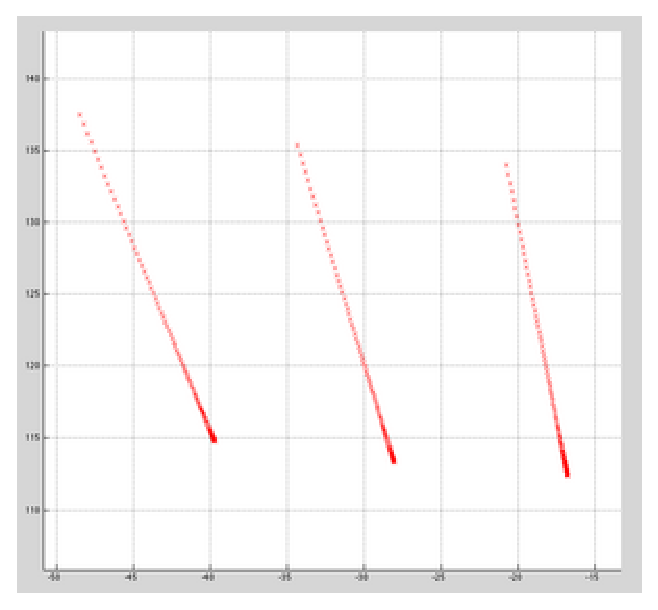
\includegraphics[width=1.65in]{isocenter/images/simulation/axial_tube_distortion_0.eps}}}
    \centerline{\emph{(b) Enlarged axial view.}}\medskip
  \end{minipage}
  \hfill
  \begin{minipage}[b]{1.65in}
    \centering
    \centerline{\mbox{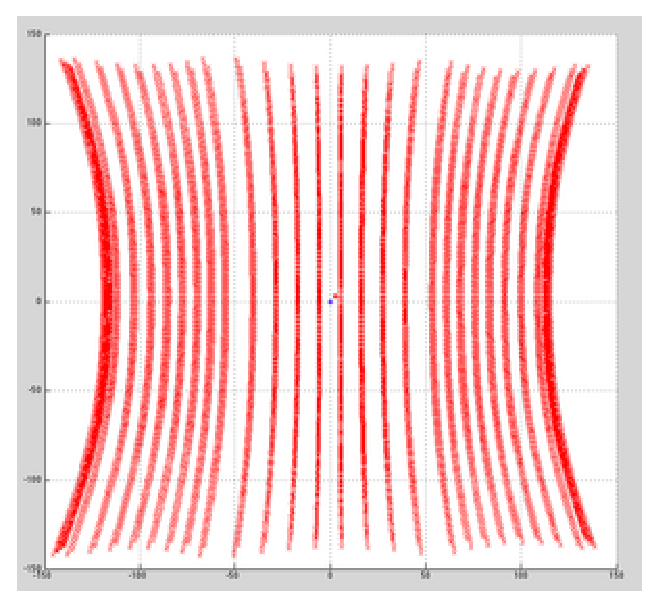
\includegraphics[width=1.65in]{isocenter/images/simulation/coronal_distortion_0.eps}}}
    \centerline{\emph{(c) Coronal view.}}\medskip
  \end{minipage}
%\hfill
%
  \caption{Phantom modeling with large distortions}
  \label{fig:2}
%
\end{figure}

\begin{figure}[htb]

  \begin{minipage}[b]{1.65in}
    \centering
    \centerline{\mbox{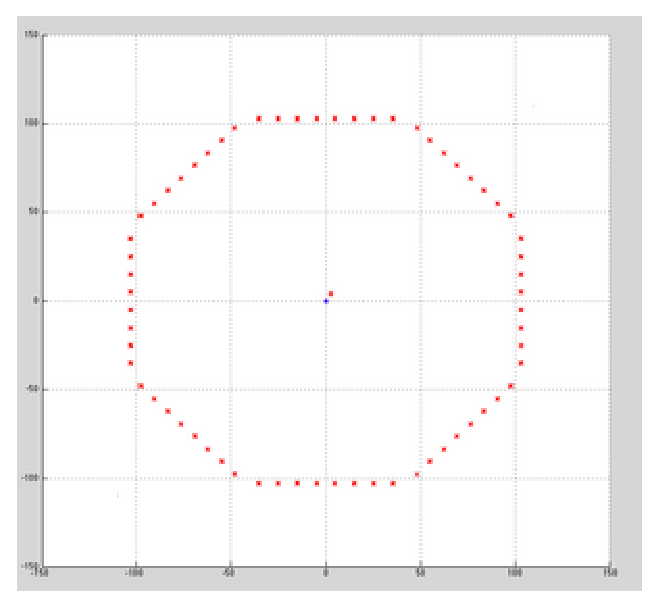
\includegraphics[width=1.65in]{isocenter/images/simulation/axial_distortion_1.eps}}}
    \centerline{\emph{(a) Axial view.}}
  \end{minipage}
  \hfill
  \begin{minipage}[b]{1.65in}
    \centering
    \centerline{\mbox{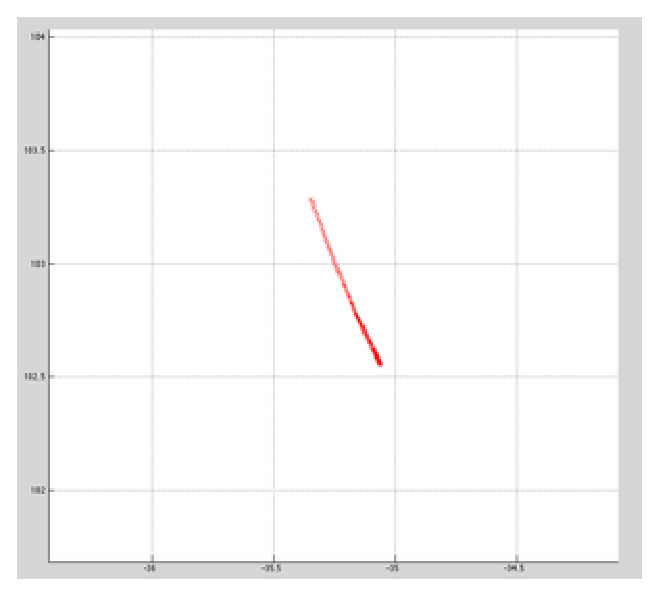
\includegraphics[width=1.65in]{isocenter/images/simulation/axial_tube_distortion_1.eps}}}
    \centerline{\emph{(b) Enlarged axial view.}}
  \end{minipage}
  \hfill
  \begin{minipage}[b]{1.65in}
    \centering
    \centerline{\mbox{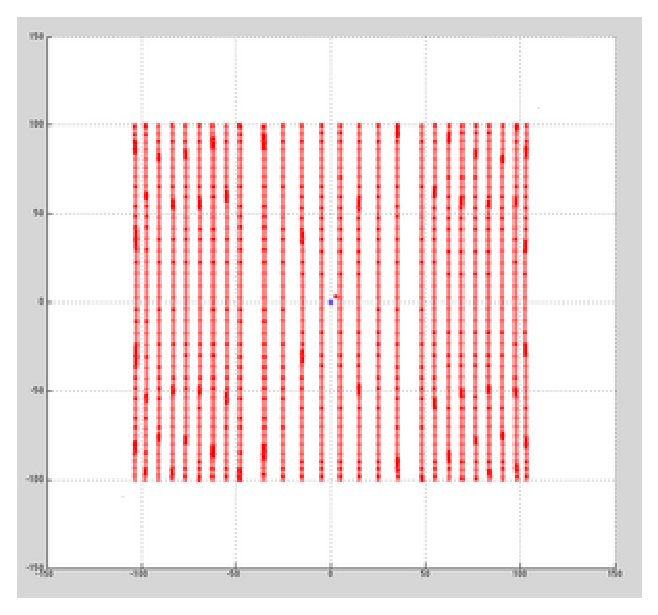
\includegraphics[width=1.65in]{isocenter/images/simulation/coronal_distortion_1.eps}}}
    \centerline{\emph{(c) Coronal view.}}
  \end{minipage}
%\hfill
%
  \caption{Phantom modeling with small distortions}
  \label{fig:3}
%
\end{figure}



Distortion in the sum of spherical harmonics is coupled in the x and y directions (orthogonal to axis), making the z axis independent.  Noise and distortion are thus very different in the z direction as opposed to the x-y plane.  We break down the gradient isocenter coordinate estimation into two big steps: estimation of z coordinate and estimation of x,y coordinate.

\subsubsection{Z-Coordinate Estimation}

Since the distortion model is based on sum of spherical harmonics, the shape of the distorted data for each tube is an even polynomial function. Figure~\ref{fig:3} shows that the realistic distortion is quite small, being about a maximum of 2 pixels, and the smaller the distortion the more sensitive the problem becomes.  With the first four terms of sum of spherical harmonics, the shape of the each tube can be seen as part of a polynomial function of 4th degree. Since the data points of tubes only represent the middle section of the 4th degree polynomial function, it is also very similar to a shape of quadratic function.  The offset between the largest distortion and the smallest distortion can be as small as 1mm.  With such a small margin, it is more practical to fit the data points to simpler model than a 4th degree polynomial.  Only the first spherical harmonic is needed in order to estimate the point where gradient is zero to measure the isocenter.  Furthermore, the first term of the sum of spherical harmonics has the largest signal to noise ratio, so we use a quadratic model to fit the data points.

We can see the distorted tube models' middle part is bending toward the center with both end bending outward.
If we were to fit each tubes to a parabola and locate the point where its gradient is zero, that point's
z-coordinate should be the same as the z-coordinate of the gradient isocenter of the magnetic field.  The z-coordinate is measured for all 64 tubes and the result averaged.  The resulting estimation is within $0.1$ mm of the actual z-coordinate.

\subsubsection{X,Y Coordinate Estimation}

The estimation of the x and y coordinates of the isocenter is the more difficult problem.
We are assuming that the difference between the distortion on x and y direction are so small that we can
treat them as if they are the same.  When this is not true, the errors on the isocenter location will be asymmetric, and it will be even more important to maintain a good numerical method to estimate the isocenter.  With that in mind, the distorted data of a tube should all stay on a plane which isocenter is also in. The intersection of such planes from each tube should be a line that
goes through isocenter. Using the isocenter estimated from previous step we should obtain an estimation
of x and y coordinate.

Since the tubes were aligned to the z-axis to reduce magnetic field distortion by the tubes, the range of data in the z-direction is of necessity larger.  In the x-y plane the range of points is controlled by the distortion, and is thus only a few pixels.  The resulting equations are highly sensitive, requiring careful handling in our numerical algorithm.

The equation of a plane in three dimensions is as follows.
\begin{eqnarray}
ax + by + cz + d & = & 0 \label{eq:plane}
\end{eqnarray}

Rewriting eq~\ref{eq:plane} with the measured data, we can solve for the plane each tube lies in.  This in turn can be used to find the intersection of the planes, which is the isocenter.
\begin{eqnarray}
-\frac{b}{a}y - \frac{c}{a}z - \frac{d}{a} & = & x \label{eq:x_orient}\\
\begin{bmatrix}
  y_0  & z_0 & 1 \\
  \vdots & \vdots & \vdots \\
  y_n & z_n & 1 \\
\end{bmatrix}
\begin{bmatrix}
-b/a\\
-c/a\\
-d/a
\end{bmatrix}
& = &
\begin{bmatrix}
x_0 \\
\vdots\\
x_n
\end{bmatrix} \nonumber\\
-m_x & = & \frac{b}{a} \nonumber\\
 k_x & = & - \frac{c}{a}z_{iso} - \frac{d}{a} \nonumber\\
  x  & = & -m_x y + k_x \nonumber\\
\begin{bmatrix}
1 \; m_x
\end{bmatrix}
\begin{bmatrix}
x \\
y
\end{bmatrix}
& = &
k_x \label{eq:x_est}
\end{eqnarray}

Note that eq~\ref{eq:plane} can be rewritten so either x or y is independent, which affects the error in standard least squares.  This becomes particularly important when the non-linearity is not the same in the x and y directions, as scaling is also well known to cause problems for least squares.
\begin{eqnarray}
-\frac{a}{b}y - \frac{c}{b}z - \frac{d}{b} & = & y \label{eq:y_orient}\\
\begin{bmatrix}
  x_0  & z_0 & 1 \\
  \vdots & \vdots & \vdots \\
  x_n & z_n & 1 \\
\end{bmatrix}
\begin{bmatrix}
-a/b\\
-c/b\\
-d/b
\end{bmatrix}
& = &
\begin{bmatrix}
y_0 \\
\vdots\\
y_n
\end{bmatrix} \nonumber\\
-m_y & = & \frac{a}{b} \nonumber\\
 k_y & = & - \frac{c}{b}z_{iso} - \frac{d}{b} \nonumber\\
  y  & = & -m_y x + k_y \\
\begin{bmatrix}
1 \; m_y
\end{bmatrix}
\begin{bmatrix}
y \\
x
\end{bmatrix}
& = &
k_y \label{eq:y_est}
\end{eqnarray}


% \begin{eqnarray}
% -\frac{a}{b}y - \frac{c}{b}z - \frac{d}{b} & = & y
% \end{eqnarray}

As we can see from figure~\ref{fig:4}, by using equation~\ref{eq:x_orient} and equation~\ref{eq:y_orient} to estimate
planes in figure~\ref{fig:4}(b) and \ref{fig:4}(d) respectively we get and quite accurate x and y coordinate
estimate. However, when you swap the choice of equations, even though they are mathematically identical,
they make a huge numeric difference as shown in \ref{fig:4}(a) and \ref{fig:4}(b).

\begin{figure}[htb]

  \begin{minipage}[b]{0.48\linewidth}
    \centering
    \centerline{\mbox{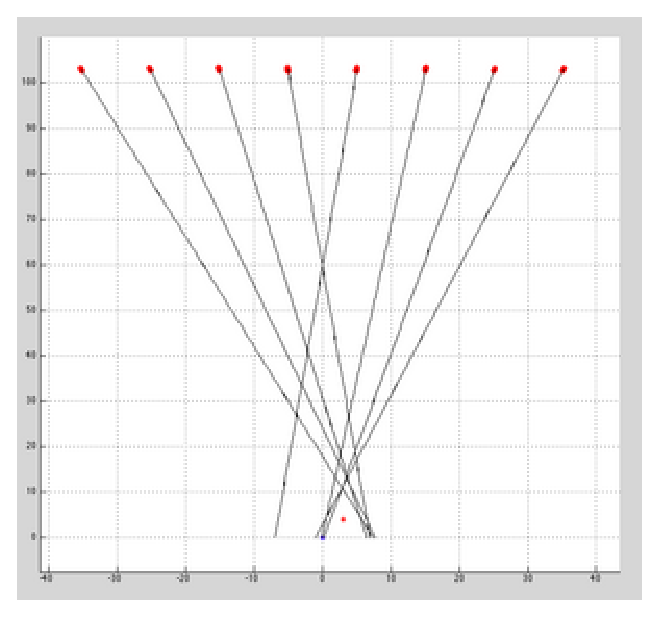
\includegraphics[width=1.65in]{isocenter/images/simulation/tube_plane_large_error_y.eps}}}
    \centerline{\emph{(a) LS fit with y orientation.}}\medskip
  \end{minipage}
  \hfill
  \begin{minipage}[b]{0.48\linewidth}
    \centering
    \centerline{\mbox{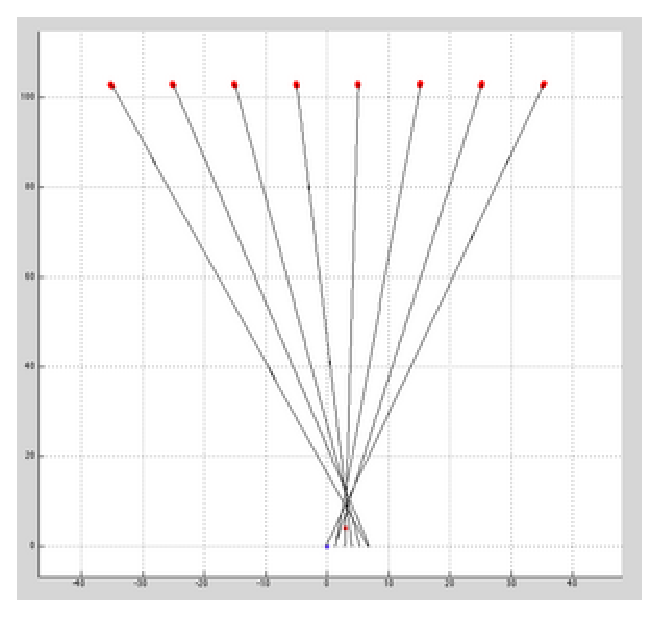
\includegraphics[width=1.65in]{isocenter/images/simulation/tube_plane_small_error_x.eps}}}
    \centerline{\emph{(b) LS fit with x orientation.}}\medskip
  \end{minipage}
  \begin{minipage}[b]{0.48\linewidth}
    \centering
    \centerline{\mbox{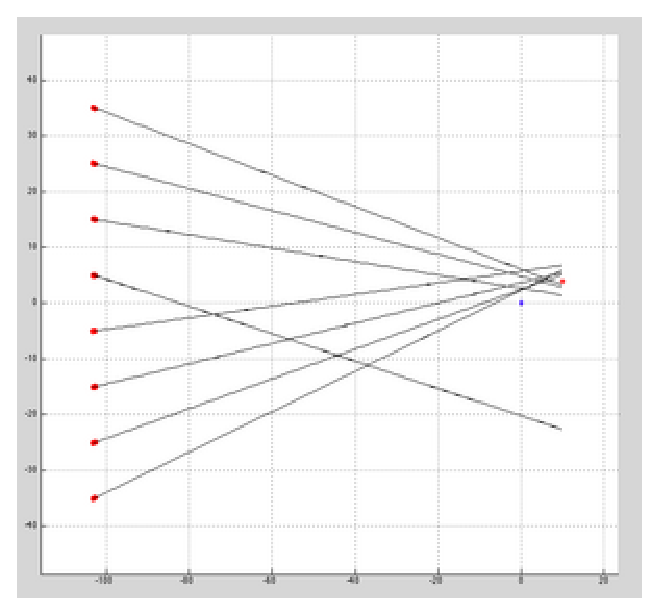
\includegraphics[width=1.65in]{isocenter/images/simulation/tube_plane_large_error_x.eps}}}
    \centerline{\emph{(c) LS fit with x orientation.}}\medskip
  \end{minipage}
  \hfill
  \begin{minipage}[b]{0.48\linewidth}
    \centering
    \centerline{\mbox{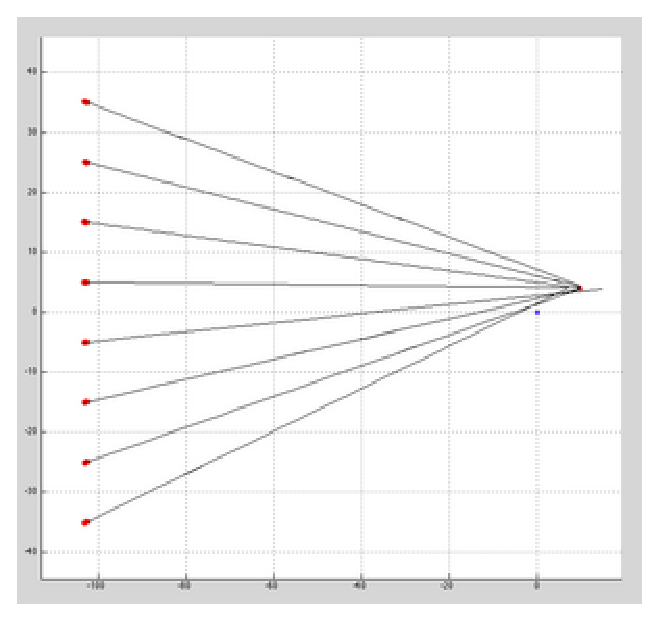
\includegraphics[width=1.65in]{isocenter/images/simulation/tube_plane_small_error_y.eps}}}
    \centerline{\emph{(d) LS fit with y orientation.}}\medskip
  \end{minipage}
  \caption{Phantom modeling with distortion, showing differences in isocenter estimates due to how the LS equation is oriented.} 
  \label{fig:4}
%
\end{figure}

When estimating the x-y coordinate using least square we should keep in mind that least square assumes
there is no observation error, it will only try to correct one side of the equation depending on how it
is setup. With this in mind, we uses equation \ref{eq:x_est} for x coordinate estimation and \ref{eq:y_est}
for y estimation. For the tubes on the diagonal planes, as we can see in fig\ref{fig:diagonal},
they offers neither a good data for x nor y coordinate estimation as compared to fig~\ref{fig:4} (b) and (d). So in order to utilize the diagonal
tubes we have to rotate these tubes to either x or y plane, and get an estimation of a rotated x-y
coordinate, then rotate the rotated x-y coordinate back and average it with original x-y coordinate
estimation.

\begin{figure}[htb]

  \begin{minipage}[b]{0.48\linewidth}
    \centering
    \centerline{\mbox{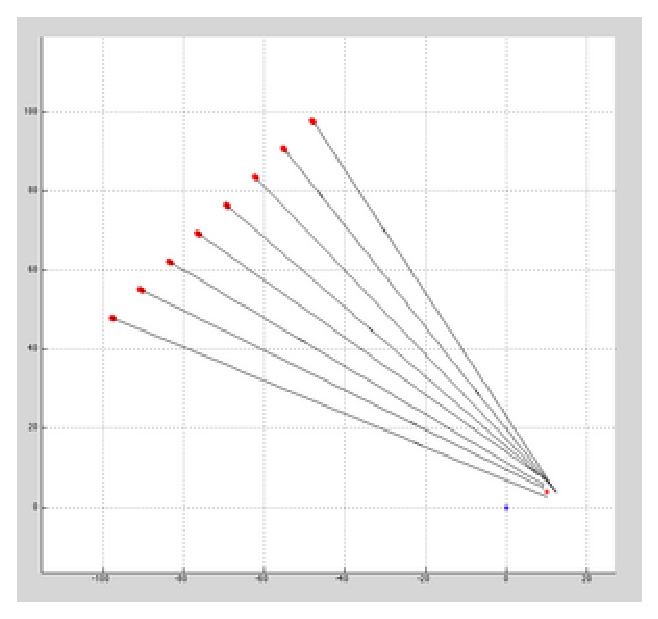
\includegraphics[width=1.65in]{isocenter/images/simulation/tube_plane_diagonal_using_x.eps}}}
    \centerline{\emph{(a) LS using x orientation.}}\medskip
  \end{minipage}
  \hfill
  \begin{minipage}[b]{0.48\linewidth}
    \centering
    \centerline{\mbox{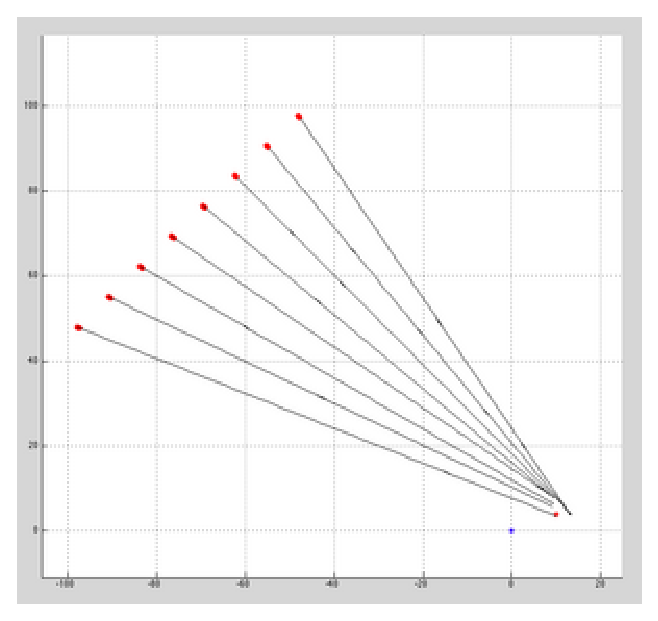
\includegraphics[width=1.65in]{isocenter/images/simulation/tube_plane_diagonal_using_y.eps}}}
    \centerline{\emph{(b) LS using y orientation.}}\medskip
  \end{minipage}
  \caption{Phantom modeling with distortion, showing how diagonal tube planes without rotation do not improve the estimates produced.} 
  \label{fig:diagonal}
%
\end{figure}

In order to obtain a good estimate, we thus must separate the estimation of x and y, as well as rotate the diagonal oriented tube planes and then separate the estimation of x and y and rotate back.  We refer to this algorithm as Rotated
Separable Least Squares (RSLS). We now present the RSLS algorithm to estimate x-y coordinate of gradient isocenter as follows:

\begin{enumerate}
\item Use equation~\ref{eq:x_orient} to estimate tube planes for tubes at upper and lower surfaces.
\item Solve equation~\ref{eq:x_est} for x and y, but only use x for x coordinate.
\item Use equation~\ref{eq:y_orient} to estimate tube planes for tubes at left and right surfaces.
\item Solve equation~\ref{eq:y_est} for y and x, but only use y for y coordinate.
\item Rotate diagonal tubes $\pi/4$, and repeat steps 1-4.
\item Rotate x-y coordinate obtained from previous step by $-\pi/4$.
\item Average the x-y coordinate from previous step with x-y coordinate calculated from step 2 and step 4 for final x-y estimation.
\end{enumerate}

Alternatively, after obtaining the plane equation parameters we can put everything into one matrix and do
a one time estimation using either least square or total least square. In table~\ref{table:symmetric}, we
can see the comparison of accuracy of estimating an isocenter at $[4 \; 4\; 3]$ using different methods.
Least square tends to lean toward one coordinate
more depends on setup, while total least square has an accurate and very balanced result due to the property
that it will try to correct errors on both side of the equation. In the contrast, our method has best
properties of both methods:

\begin{itemize}
  \item It is accurate. For both x and y coordinate it does a better job than total least square, much better than least square's worst case and very close to least square's best case.
  \item It has very balanced result. Both x and y coordinates are very close the correct result equally just like total least square.
  \item It has very tight error boundaries. After 200 runs, it's error is tighter than standard least square.
\end{itemize}

Therefore, our estimation method is a good alternative to traditional least square or total least square methods. Although it might require more computation, it could be easily dealt by modern GPU computing. And due to the fact that each least square estimation has relative small matrix, and each estimation is independent of each other, it is very close to ``embarrassingly parallel'' type of problems and makes it easy to solve.


%KES the other is too nice for all examples so we need to show the ugliness.  I don't have the data, so I am setting what
%    I recall from our talk last night.  It will need your data.

In table~\ref{table:symmetric}, the test is run using a symmetric x-y axis distortion. We can see that all three methods performed very well. RSLS method's result is slightly better than Total Least Squares (TLS), and one on y axis it is better than standard Least Squares method.

%KES - what is two LS method and what is one LS method?  must explain in text?
%      is one traditional and the other our new method?
\begin{table}
  \begin{tabular} {| l | r | r | r | r | r | r |}
    \hline
    & $\bar{x}$ & $\sigma_x$ & err & $\bar{y}$ & $\sigma_y$ & err  \\
    \hline
    RSLS  & 3.9709 & 0.1068  & 0.0291 & 3.9677 & 0.1008 & 0.0323\\
    \hline
    LS & 3.9950 & 0.1118 & 0.0050   & 3.9414 & 0.1011 & 0.0586 \\
    \hline
    TLS  & 4.0800 & 0.1035  & 0.0800   & 4.0800 & 0.0964 & 0.0800 \\
    \hline
  \end{tabular}
  \caption{Average of 200 runs using different methods for estimating the isocenter at $[4 \; 4 \; 3]$ in the presence of symmetrical distortion} 
  \label{table:symmetric}
\end{table}


When the distortion is not symmetrical the issue of proper estimation becomes crucial. In table~\ref{table:nonsymmetric}, we show the result of using non-symmetrical distortion in which the y direction was set to be twice the distortion in the x. In this test, TLS method's result is the worst, off by a few millimeters.  Both LS and RSLS show comparable degradation of performance in x.  LS shows degradation in the estimation of y as well, but RSLS, since it is separable, does not experience any degradation of it. Only the RSLS's result remains quite accurate. This shows the advantage of RSLS over the other two traditional methods.


\begin{table}
  \begin{tabular} {| l | r | r | r | r | r | r |}
    \hline
    & $\bar{x}$ & $\sigma_x$ & err & $\bar{y}$ & $\sigma_y$ & err \\
    \hline
    RSLS & 3.8073 & 0.1117 & 0.1927   & 3.9838 & 0.1059 & 0.0162 \\
    \hline
    LS  & 4.2191 & 0.1117    & 0.2191 & 3.8765 & 0.1003 & 0.1235 \\
    \hline
    TLS  & 9.5744 & 0.2616 & 5.5744   & 8.6905 & 0.2393 & 4.6905 \\
    \hline
  \end{tabular}
  \caption{Average of 200 runs using different methods for estimating the isocenter at $[4 \; 4 \; 3]$ in the presence of non-symmetrical distortion } 
  \label{table:nonsymmetric}
\end{table}


\section{Conclusion}
In this work, we developed a new numerical algorithm to accurately determine the gradient isocenter
of MRI scanners based on a new distortion correction phantom. Knowledge of the gradient isocenter is an essential part of gradient-nonlinearity correction methods.  We have shown that the method used in this work to estimate the gradient isocenter is a good alternative to more traditional estimation methods such as least squares and total least squares. The new algorithm is particularly suited when the image data are extremely sensitive to the presence of noise and asymmetric distortion. Using simulated (but realistic) distortion data, it was shown, that the resulting estimated isocenter was within $0.2$ mm of the actual gradient isocenter, leading to a better estimate than the currently used DICOM coordinate center.
